\documentclass[aspectratio=169]{beamer}
\usepackage{lmodern}
%\usetheme{Madrid}
%\usecolortheme{giantoak}
\newcommand*\oldmacro{}
\let\oldmacro\insertshorttitle
\renewcommand*\insertshorttitle{\oldmacro\hfill\insertframenumber\,/\,\inserttotalframenumber}
\usepackage[framemethod=tikz]{mdframed}

%\usepackage{beamerthemesplit}
\usepackage{textpos}
\usepackage{pgf}
\usepackage{ulem}
%\logo{\pgfputat{\pgfxy(0,-.4)}{\pgfbox[right,base]{\includegraphics[height=1.0cm]{logo.jpg}}}}
%\newcommand{\nologo}{\setbeamertemplate{logo}{}}
\usepackage{booktabs}
\usepackage{graphicx}
\theoremstyle{principle}
\newtheorem*{principle}{Design Principle}


\titlegraphic{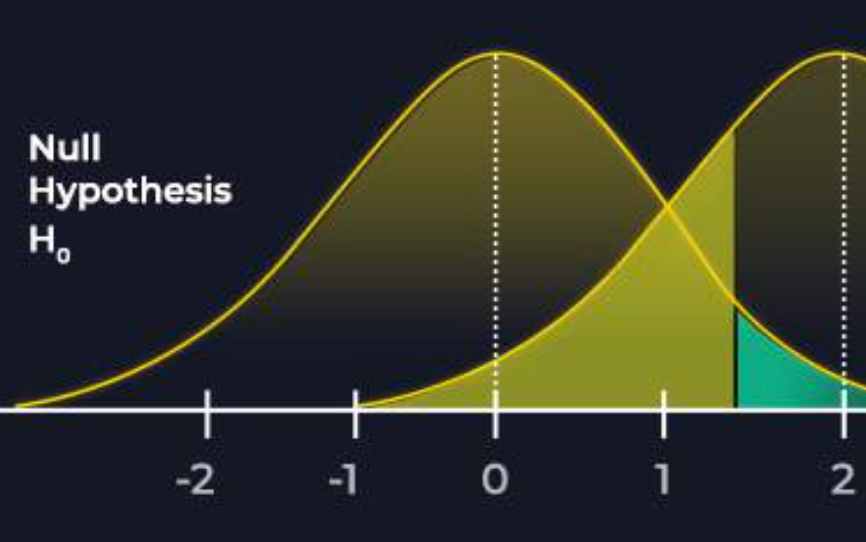
\includegraphics[width=1.0\paperwidth]{distros.png}}

\title{Amendments}
%\author[Jeremy Kedziora]{Wind Data Science Team\\
%\small{Uptake}}
\date{}

\begin{document}

%{
%%\nologo
%\begin{frame}
%    \maketitle
%\end{frame}
%}
%pages 1-7, 8-9, 14-15.


{
%  \usebackgroundtemplate{
\includegraphics[width=1.0\paperwidth]{statistics-review.jpg}}
  \usebackgroundtemplate{
\includegraphics[scale=0.7]{poll860.jpg}}
  \begin{frame}[plain]
  
\begin{mdframed}[tikzsetting={draw=white,fill=white,fill opacity=0.6,draw opacity=0.4,
               line width=0pt},backgroundcolor=none,leftmargin=20,
               rightmargin=20,innertopmargin=4pt]
\begin{center}
\Huge \textbf{Political Polling}
\end{center}
\end{mdframed}

  \end{frame}
}

%most reliant on human cognition
%limited only by cognition
%hypothesis generating scheme often functioning as a gateway into more statistical analysis

%%@@@@@@@@@@@@@@@@@@@@@@@@@@@@@@@@@@@@@@@@@@@@@@@@@
%\begin{frame}
%\frametitle{Napoleon's Progress}
%\begin{center}
%
\includegraphics[scale=0.4]{experiment.png}
%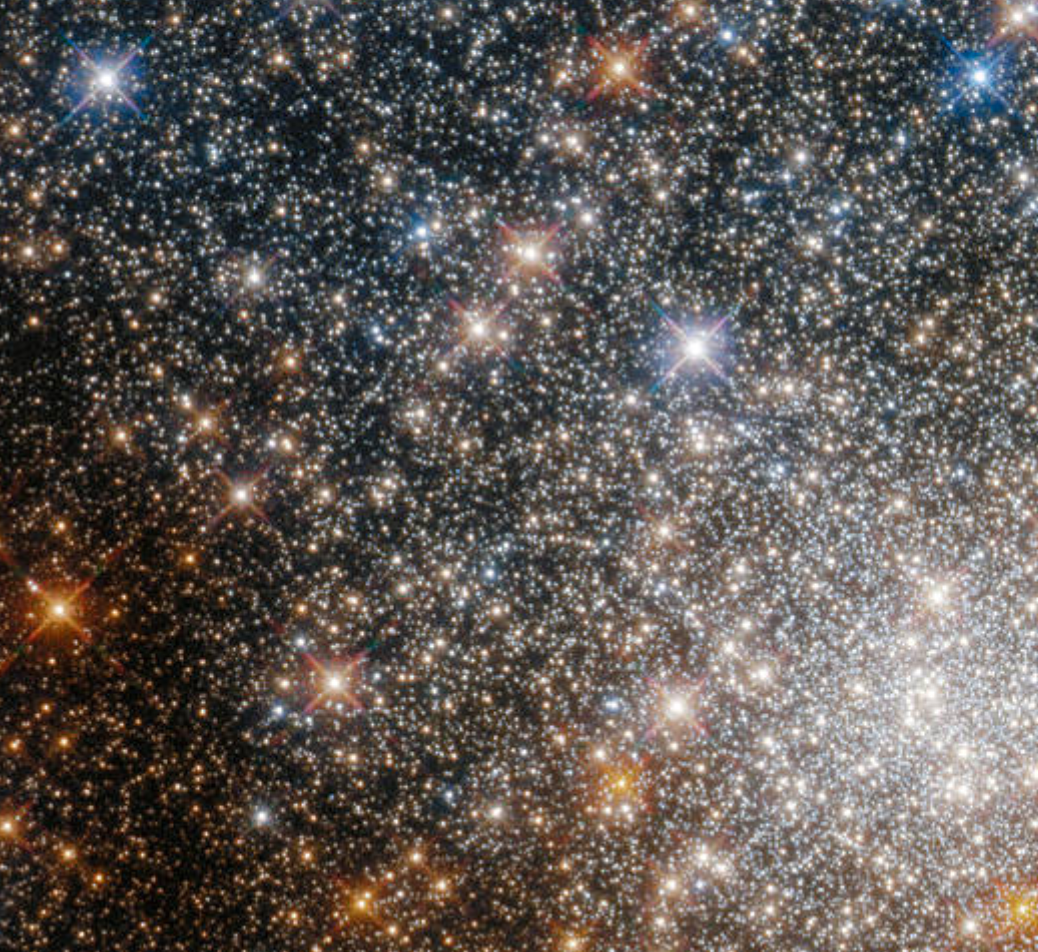
\includegraphics[scale=0.35]{stars.png}
%\end{center}
%
%\end{frame}

%@@@@@@@@@@@@@@@@@@@@@@@@@@@@@@@@@@@@@@@@@@@@@@@@@
\begin{frame}
\frametitle{Today:}

\begin{itemize}
\item Introduce the methods associated with polling;
\bigskip
\bigskip
\bigskip

\item Examine some failures;
\bigskip
\bigskip
\bigskip

\item Ask whether polls are good or not.

\end{itemize}

\end{frame}

%%@@@@@@@@@@@@@@@@@@@@@@@@@@@@@@@@@@@@@@@@@@@@@@@@@
%\begin{frame}
%\frametitle{Building blocks}
%
%\begin{columns}
%\begin{column}{0.5\textwidth}
%
%\begin{itemize}
%\item FiveThirtyEight uses fundamentals (and historical data) to build ``prior expectations" for Election Day;
%\begin{itemize}
%\item Anchors each state as the model projects to Election Day;
%\item Explores how each state differs from the average;
%\item When state predictions are wrong, allows assessment of which states are ``wrong together;"
%\end{itemize}
%\bigskip
%
%\item New polls ``update our prior expectations" about Election Day.
%\end{itemize}
%
%\end{column}
%\begin{column}{0.5\textwidth}
%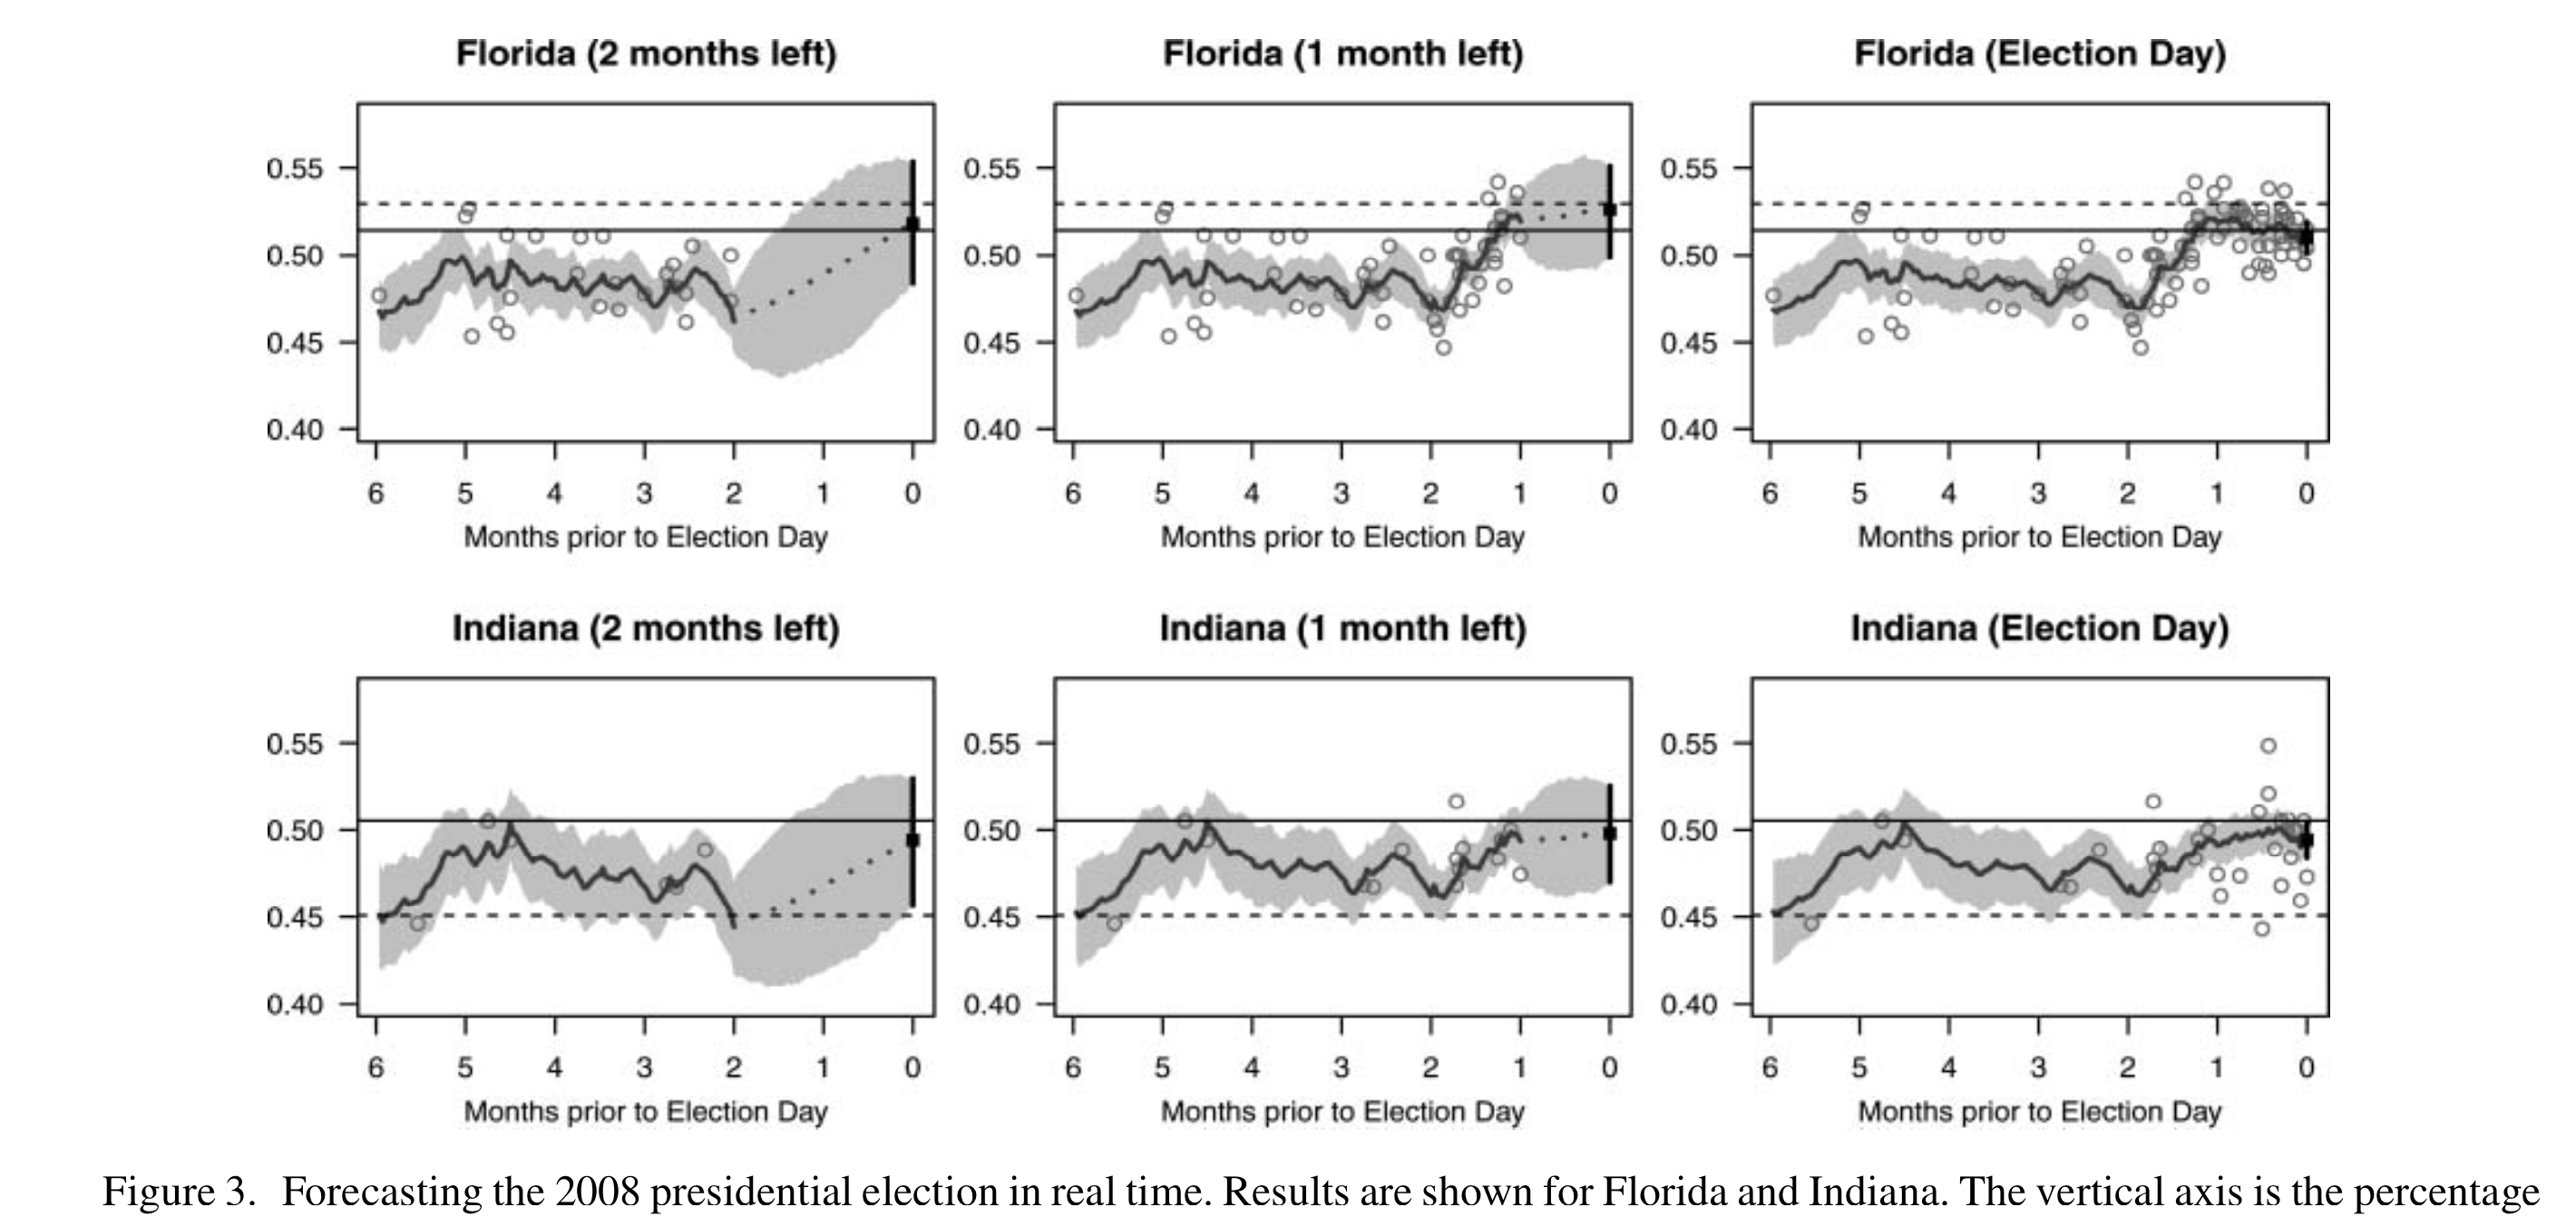
\includegraphics[scale=0.15]{random-walk.png}
%\end{column}
%\end{columns}
%
%\end{frame}

%@@@@@@@@@@@@@@@@@@@@@@@@@@@@@@@@@@@@@@@@@@@@@@@@@
\begin{frame}
\frametitle{What is opinion polling?}

\begin{center}
\Huge \textbf{A series of questions given to a group to learn about them through the answers.}
\end{center}

\end{frame}

%@@@@@@@@@@@@@@@@@@@@@@@@@@@@@@@@@@@@@@@@@@@@@@@@@
\begin{frame}
\frametitle{What is opinion polling?}

\begin{itemize}
\item \textbf{Benchmark poll} -- before campaigning begins, sort of like the control in a within subject experimental design;
\bigskip

\item \textbf{Tracking poll} -- a poll conducted over time, summarized as a moving average;
\bigskip

\item \textbf{Brushfire poll} -- used by a campaign to test a message or strategy on a limited audience;
\bigskip

\item \textbf{Straw poll} -- issue focused, usually a non-statistical attempt to learn about where people stand;
\bigskip

\item \textbf{Entrance/Exit poll} -- conducted immediately before/after voting;
\bigskip

\item \textbf{Push poll} -- a poll used to influence, e.g. through question wording or timing.
\end{itemize}

\end{frame}

%@@@@@@@@@@@@@@@@@@@@@@@@@@@@@@@@@@@@@@@@@@@@@@@@@
\begin{frame}
\frametitle{Sampling methodology}

\begin{itemize}
\item \textbf{Representative sample}: a sample is representative if its characteristics ``look like" the population;
\bigskip
\item \textbf{Generalizable}: a sample is generalizable if we can make ``good" guesses about the population using the characteristics of the sample;
\bigskip
\item \textbf{Bias}: a sample is biased if certain individuals in a population have a higher chance of being included in a sample than others;
\bigskip
\item[]\color{white} In general if we create a sample of size $n$ randomly then...
\begin{itemize}
\item[]\color{white} ...the sample will be unbiased and representative of the population of size $N$ so...
\item[]\color{white} ...any result based on the sample with generalize to the population and therefore...
\item[]\color{white} ...the sample statistic is a good guess for the population parameter which means...
\item[]\color{white} ...that we can \textbf{INFER} about the population using the sample.
\end{itemize}

\end{itemize}

\end{frame}

%@@@@@@@@@@@@@@@@@@@@@@@@@@@@@@@@@@@@@@@@@@@@@@@@@
\begin{frame}
\frametitle{Sampling methodology}

\begin{itemize}
\item \textbf{Representative sample}: a sample is representative if its characteristics ``look like" the population;
\bigskip
\item \textbf{Generalizable}: a sample is generalizable if we can make ``good" guesses about the population using the characteristics of the sample;
\bigskip
\item \textbf{Bias}: a sample is biased if certain individuals in a population have a higher chance of being included in a sample than others;
\bigskip
\item In general if we create a sample of size $n$ randomly then...
\begin{itemize}
\item ...the sample will be unbiased and representative of the population of size $N$ so...
\item ...any result based on the sample with generalize to the population and therefore...
\item ...the sample statistic is a good guess for the population parameter which means...
\item ...that we can \textbf{INFER} about the population using the sample.
\end{itemize}
\end{itemize}

\end{frame}

%@@@@@@@@@@@@@@@@@@@@@@@@@@@@@@@@@@@@@@@@@@@@@@@@@
\begin{frame}
\frametitle{Margin of Error}

\begin{itemize}
\item Consider a simple poll: \textbf{``Do you plan to vote for Biden, yes/no?"}
\begin{itemize}
\item The poll has $n$ respondents;
\item We are interested in the population proportion $v_P$ that plan to vote for Biden;
\item We have the sample proportion $v_S$ that plan to vote for Biden;
\end{itemize}
\bigskip

\item We'd like to put a $\pm$ around $v_S$ -- very common to use the margin of error (another name for confidence interval) to do this;
\bigskip
\bigskip

\item Assume that $v_S$ is normally distributed around $v_P$ -- let's focus on an area that captures $95\%$ of all possible values for $v_S$;
\begin{align*}
MOE = 1.96\sqrt{\frac{v_S(1-v_S)}{n}}.
\end{align*}
\end{itemize}

\end{frame}

%@@@@@@@@@@@@@@@@@@@@@@@@@@@@@@@@@@@@@@@@@@@@@@@@@
\begin{frame}
\frametitle{Margin of Error}

\begin{itemize}
\item Consider a simple poll: \textbf{``Do you plan to vote for Biden, yes/no?"}
\begin{itemize}
\item The poll has $n$ respondents;
\item We are interested in the population proportion $v_P$ that plan to vote for Biden;
\item We have the sample proportion $v_S$ that plan to vote for Biden;
\end{itemize}
\bigskip

\item We'd like to put a $\pm$ around $v_S$ -- very common to use the margin of error (another name for confidence interval) to do this;
\bigskip
\bigskip

\item Assume that $v_S$ is normally distributed around $v_P$ -- let's focus on an area that captures $95\%$ of all possible values for $v_S$;
\begin{align*}
MOE = 1.96\sqrt{\frac{v_S(1-v_S)}{n}}.
\end{align*}
\end{itemize}

\end{frame}

%@@@@@@@@@@@@@@@@@@@@@@@@@@@@@@@@@@@@@@@@@@@@@@@@@
\begin{frame}
\frametitle{Why do polls fail?}

\begin{columns}
\begin{column}{0.5\textwidth}

\begin{itemize}
\item Not representative (e.g. selective nonresponse, collection method);
\bigskip

\item Response bias (e.g. spiral of silence);
\bigskip

\item Question wording (e.g. double negatives, implicit assumptions, etc.);
\bigskip

\item Question ordering (e.g. a `push' question can change responses to follow ups);
\bigskip

\item Polling timing (e.g. missing dynamics);

\end{itemize}

\end{column}
\begin{column}{0.5\textwidth}
\begin{center}
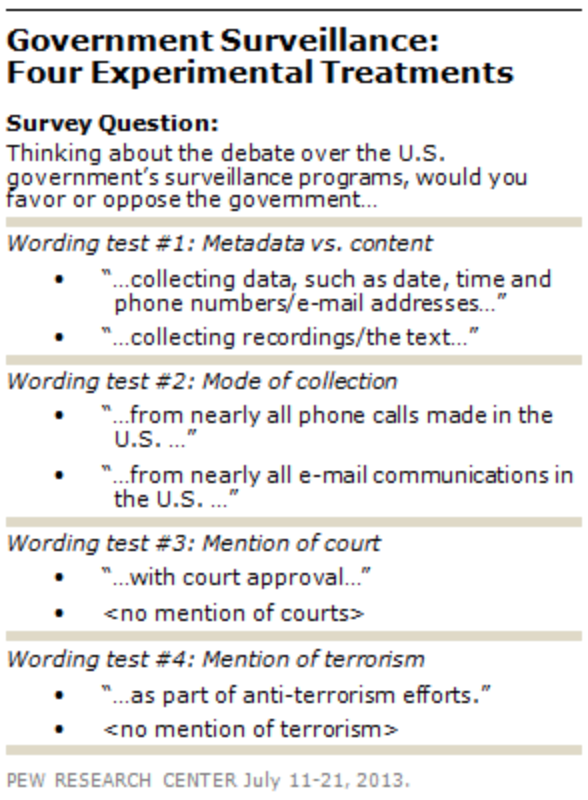
\includegraphics[scale=0.5]{pew_1.png}
\end{center}
\end{column}
\end{columns}

\end{frame}

%@@@@@@@@@@@@@@@@@@@@@@@@@@@@@@@@@@@@@@@@@@@@@@@@@
\begin{frame}
\frametitle{Why do polls fail?}

\begin{columns}
\begin{column}{0.5\textwidth}

\begin{itemize}
\item Not representative (e.g. selective nonresponse, collection method);
\bigskip

\item Response bias (e.g. spiral of silence);
\bigskip

\item Question wording (e.g. double negatives, implicit assumptions, etc.);
\bigskip

\item Question ordering (e.g. a `push' question can change responses to follow ups);
\bigskip

\item Polling timing (e.g. missing dynamics);

\end{itemize}

\end{column}
\begin{column}{0.5\textwidth}
\begin{center}
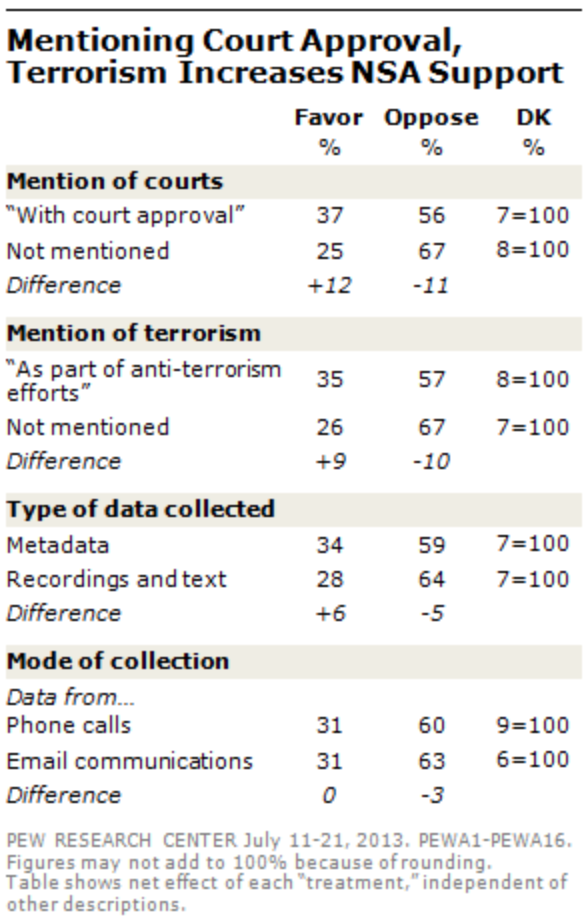
\includegraphics[scale=0.5]{pew_2.png}
\end{center}
\end{column}
\end{columns}

\end{frame}

%@@@@@@@@@@@@@@@@@@@@@@@@@@@@@@@@@@@@@@@@@@@@@@@@@
\begin{frame}
\frametitle{Failures: polling in 1936...}

\begin{columns}
\begin{column}{0.5\textwidth}

\begin{itemize}
\item \textit{The Literary Digest}:
\begin{itemize}
\item A weekly magazine that started in 1890 w/ circulation $> 1,000,000$;
\item Correctly predicted US presidential elections from 1916 -- 1932;
\end{itemize}

\item 1936 Election: Langdon v Roosevelt;
\begin{itemize}
\item \textit{The Literary Digest} polled 10 million and got 2.3 million responses;
\item Langdon predicted to be the decisive winner -- but Roosevelt crushed him!
\end{itemize}

\item The magazine folded within 18 months -- what happened?! \color{white} Sampled:
\begin{itemize}
\item[]\color{white} Auto registrations;
\item[]\color{white} Phone number lists;
\item[]\color{white} Country club memberships;
\item[]\color{white} Its own subscriber list.
\end{itemize}
\end{itemize}

\end{column}
\begin{column}{0.5\textwidth}
\begin{center}
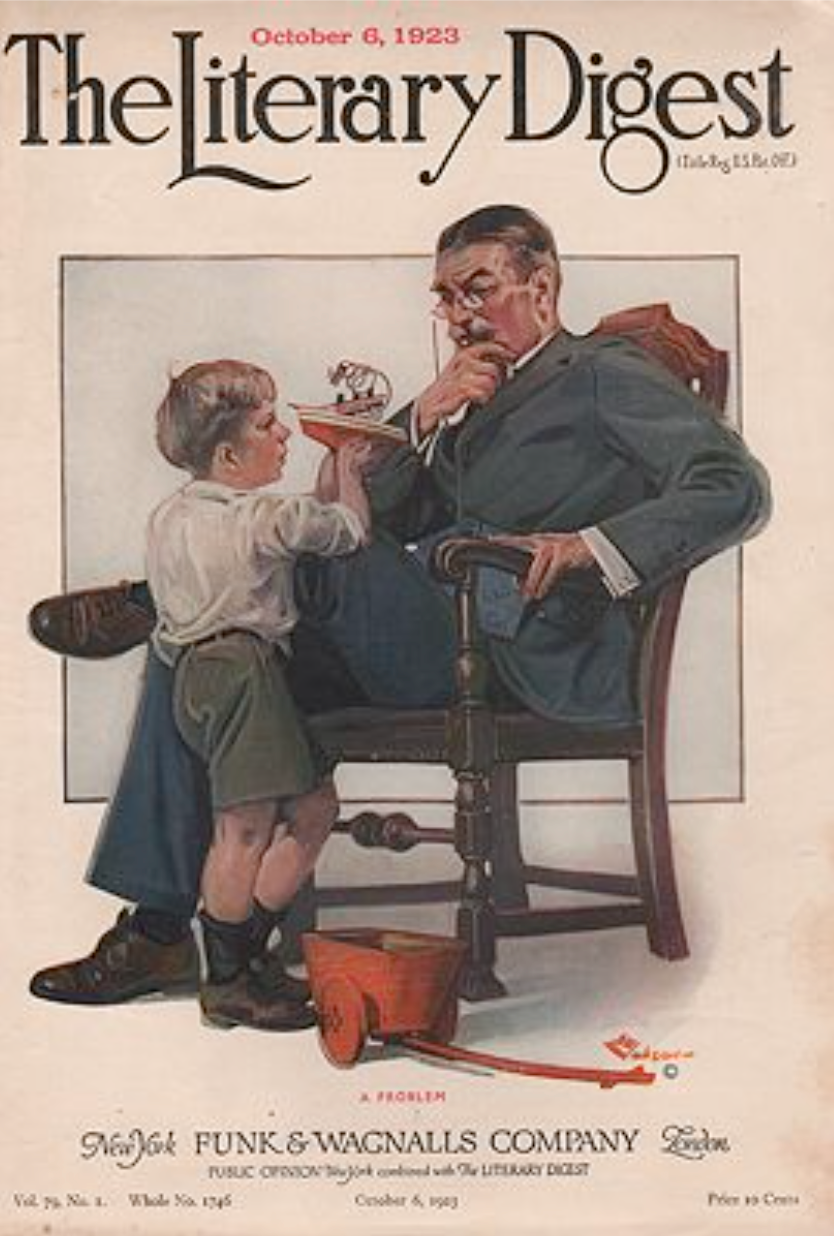
\includegraphics[scale=0.3]{LD.png}
\end{center}
\end{column}
\end{columns}

\end{frame}

%@@@@@@@@@@@@@@@@@@@@@@@@@@@@@@@@@@@@@@@@@@@@@@@@@
\begin{frame}
\frametitle{Failures: polling in 1936...}

\begin{columns}
\begin{column}{0.5\textwidth}

\begin{itemize}
\item \textit{The Literary Digest}:
\begin{itemize}
\item A weekly magazine that started in 1890 w/ circulation $> 1,000,000$;
\item Correctly predicted US presidential elections from 1916 -- 1932;
\end{itemize}

\item 1936 Election: Langdon v Roosevelt;
\begin{itemize}
\item \textit{The Literary Digest} polled 10 million and got 2.3 million responses;
\item Langdon predicted to be the decisive winner -- but Roosevelt crushed him!
\end{itemize}

\item The magazine folded within 18 months -- what happened?!  Sampled:
\begin{itemize}
\item Auto registrations;
\item Phone number lists;
\item Country club memberships;
\item Its own subscriber list.
\end{itemize}
\end{itemize}

\end{column}
\begin{column}{0.5\textwidth}
\begin{center}
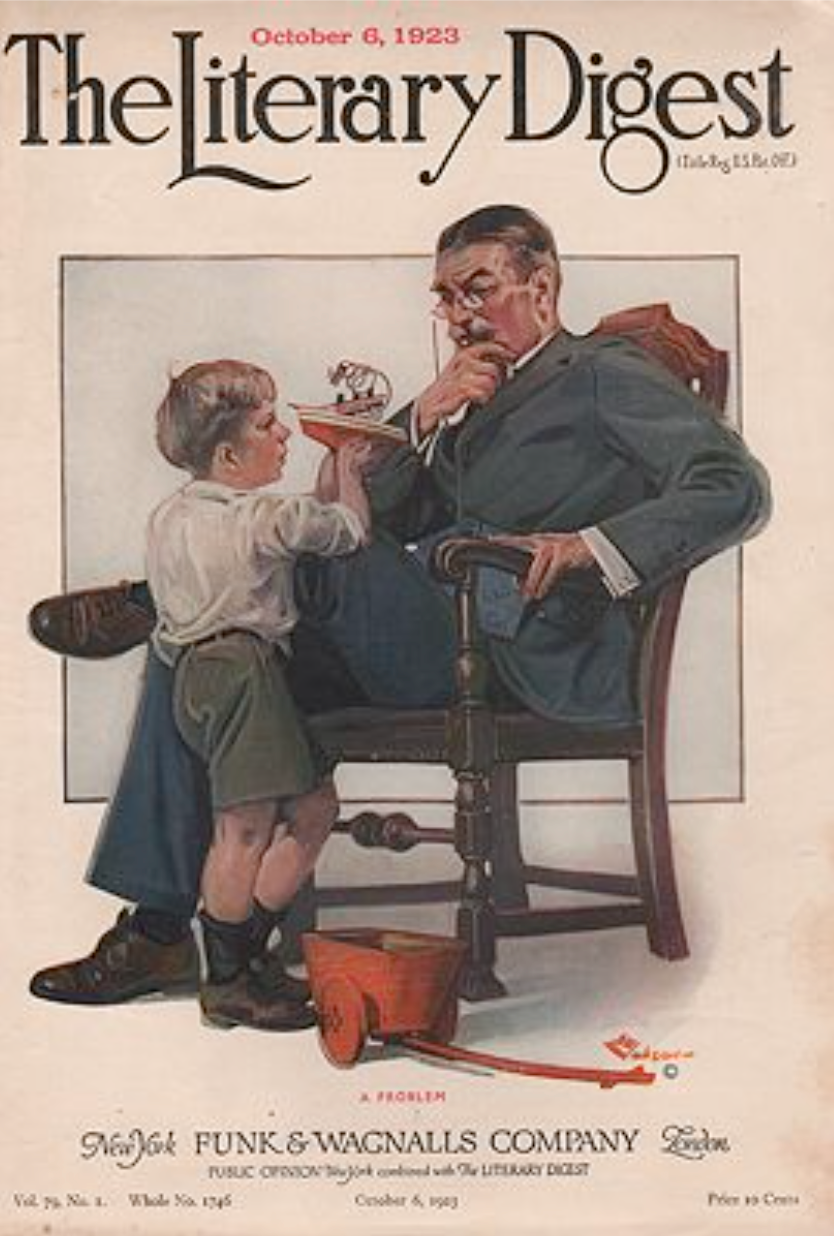
\includegraphics[scale=0.3]{LD.png}
\end{center}
\end{column}
\end{columns}

\end{frame}

%@@@@@@@@@@@@@@@@@@@@@@@@@@@@@@@@@@@@@@@@@@@@@@@@@
\begin{frame}
\frametitle{Failures: polling in 1948...}

\begin{columns}
\begin{column}{0.5\textwidth}

\begin{itemize}
\item Professional polling:
\begin{itemize}
\item Gallup founded in 1935, pioneered representative sampling;
\item Correctly choose Roosevelt in 1936;
\end{itemize}

\item 1948 Election: Truman v Dewey;
\begin{itemize}
\item Polling predicted Dewey to win convincingly;
\item At no point on election day was Truman ever behind Dewey;
\end{itemize}

\item What went wrong this time?!
\begin{itemize}
\item[]\color{white} Farley's Law: the election is decided at the time of the conventions;
\item[]\color{white} Polling dropped off end of Oct;
\item[]\color{white} Truman picked up 14\% of his voters in the two weeks before election day.
\end{itemize}
\end{itemize}

\end{column}

\begin{column}{0.5\textwidth}
\begin{center}
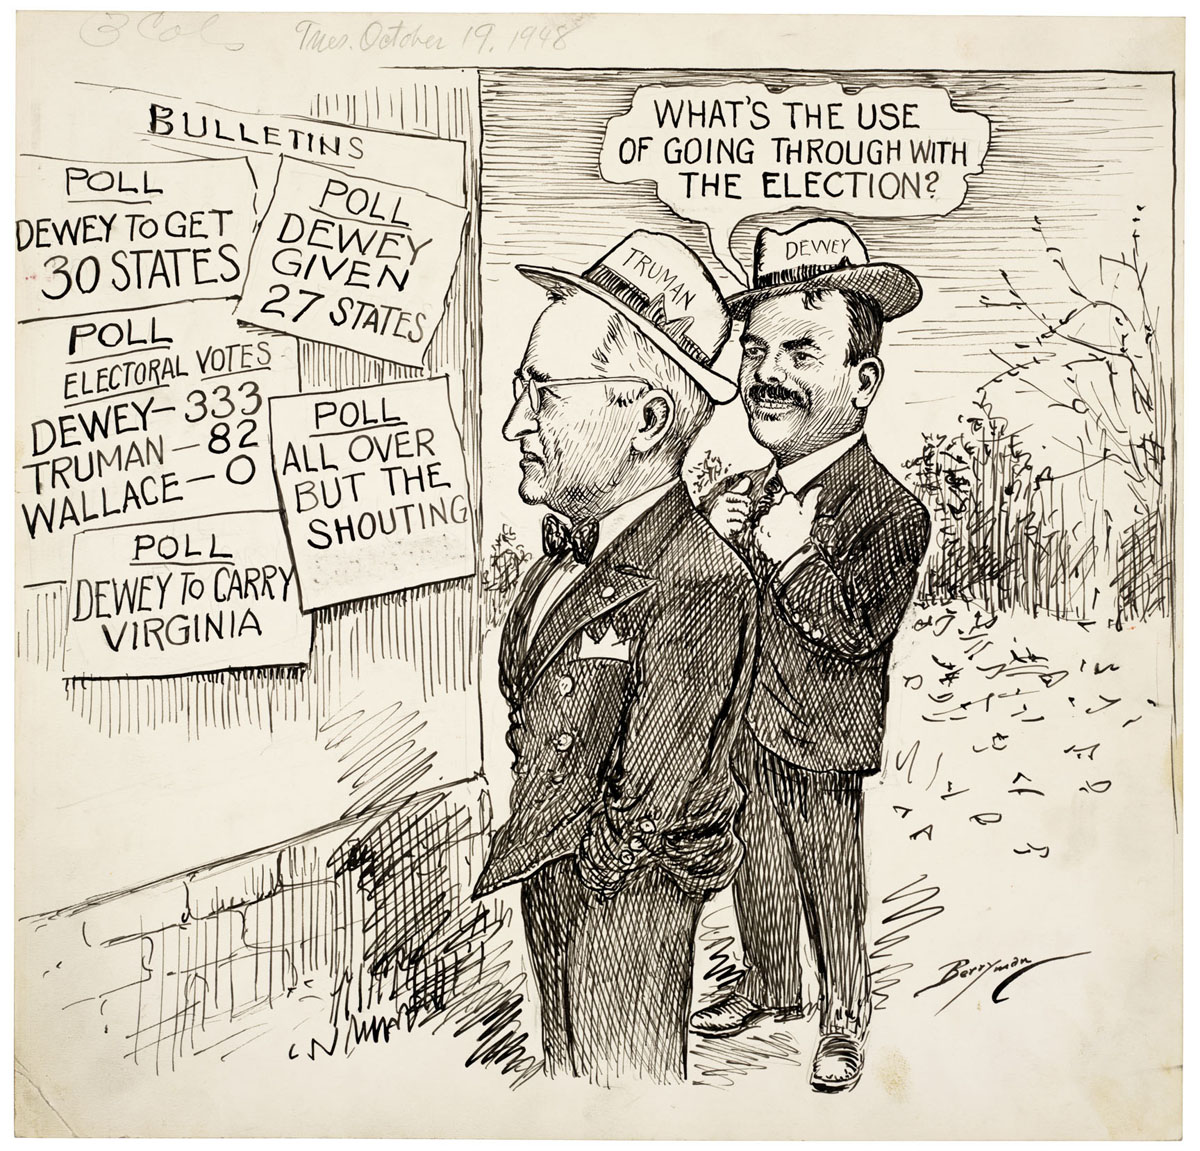
\includegraphics[scale=0.25]{Truman-Dewey-polls-1948.jpg}
\end{center}
\end{column}
\end{columns}

\end{frame}

%@@@@@@@@@@@@@@@@@@@@@@@@@@@@@@@@@@@@@@@@@@@@@@@@@
\begin{frame}
\frametitle{Failures: polling in 1948...}

\begin{columns}
\begin{column}{0.5\textwidth}


\begin{itemize}
\item Professional polling:
\begin{itemize}
\item Gallup founded in 1935, pioneered representative sampling;
\item Correctly choose Roosevelt in 1936;
\end{itemize}

\item 1948 Election: Truman v Dewey;
\begin{itemize}
\item Polling predicted Dewey to win convincingly;
\item At no point on election day was Truman ever behind Dewey;
\end{itemize}

\item What went wrong this time?!
\begin{itemize}
\item Farley's Law: the election is decided at the time of the conventions;
\item Polling dropped off end of Oct;
\item Truman picked up 14\% of his voters in the two weeks before election day.
\end{itemize}
\end{itemize}

\end{column}
\begin{column}{0.5\textwidth}
\begin{center}
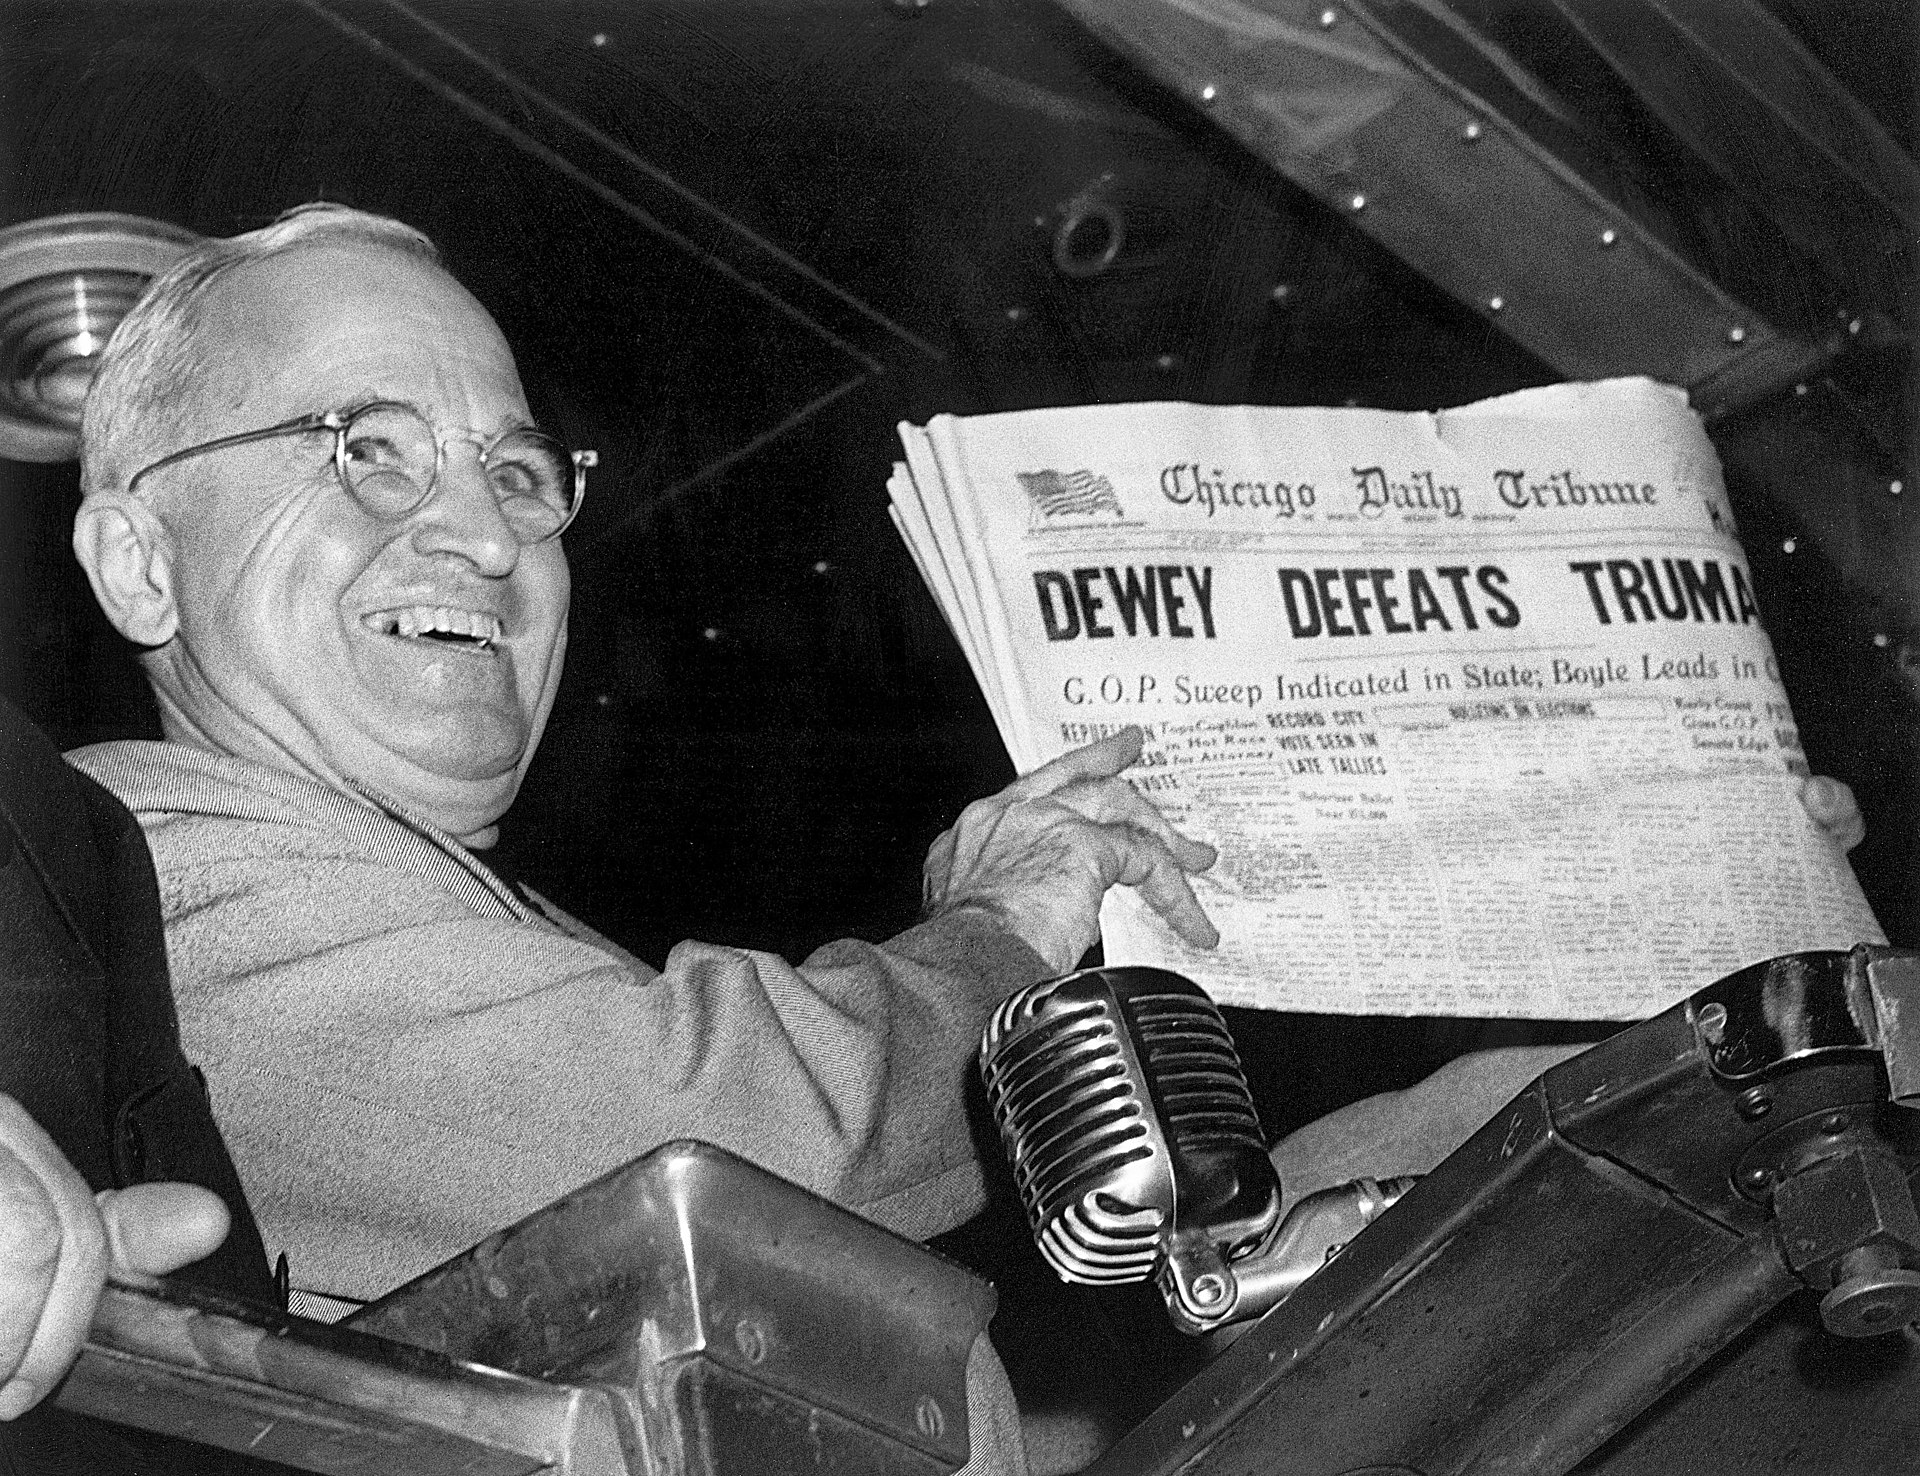
\includegraphics[scale=0.1]{Dewey_Defeats_Truman.jpg}
\end{center}
\end{column}
\end{columns}

\end{frame}

%@@@@@@@@@@@@@@@@@@@@@@@@@@@@@@@@@@@@@@@@@@@@@@@@@
\begin{frame}
\frametitle{Failures: polling in 2016...}

\begin{columns}
\begin{column}{0.5\textwidth}


\begin{itemize}
\item Election forecasting:
\begin{itemize}
\item We talked about fivethirtyeight but also NYT Upshot, Daily Kos, etc.;
\item Growth in ecosystem a reflection of recent successes;
\end{itemize}

\item 2016 Election: Clinton v Trump;
\begin{itemize}
\item Unanimity among polls/forecasts that Clinton would win;
\item We know what happened...
\end{itemize}

\item Again?!
\begin{itemize}
\item[]\color{white} Polling not representative -- too many college grads;
\item[]\color{white} Large number of undecided voters in all polls;
\item[]\color{white} Very late swing amongst undecideds towards Trump.
\end{itemize}
\end{itemize}

\end{column}
\begin{column}{0.5\textwidth}
\begin{center}
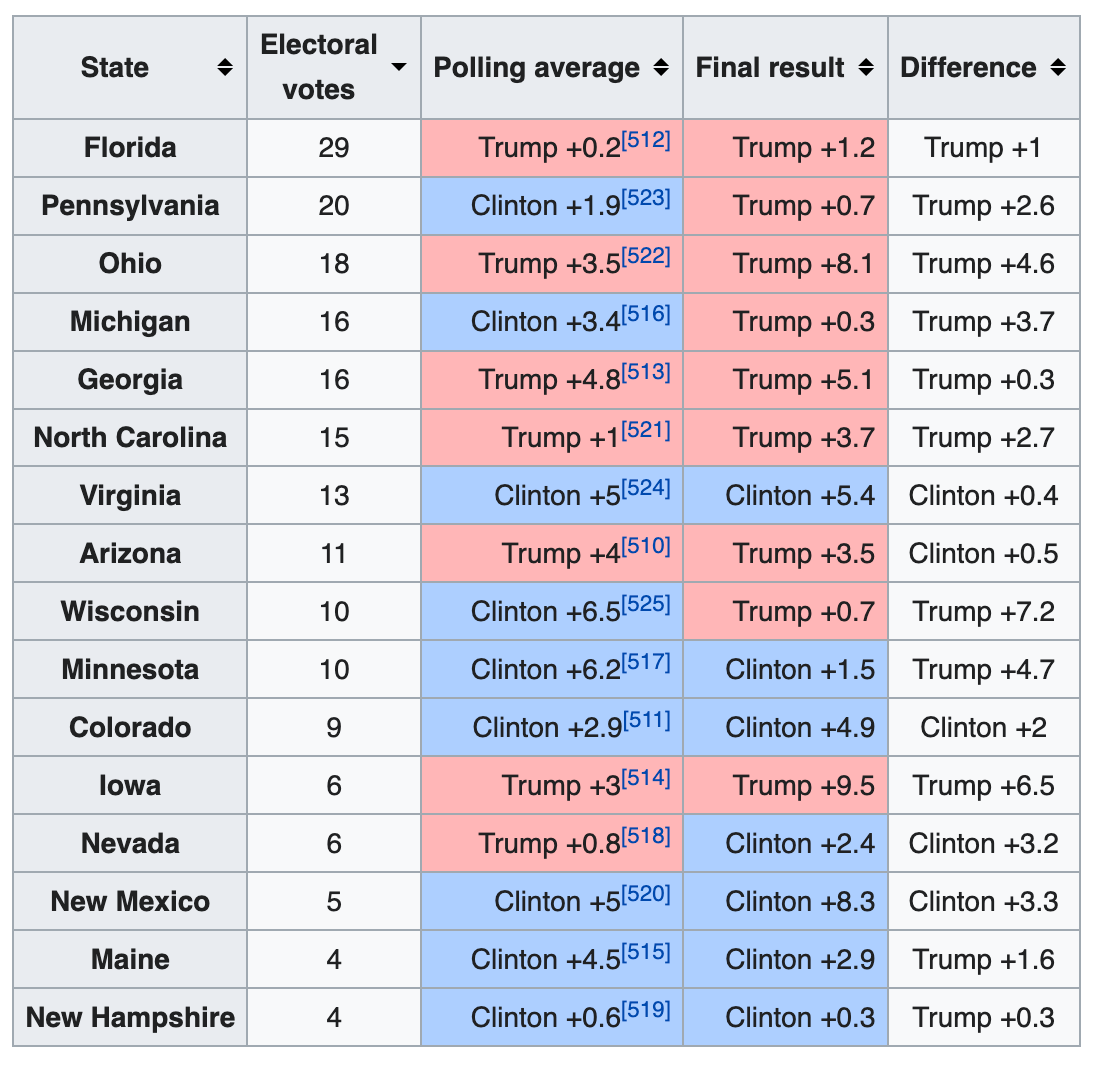
\includegraphics[scale=0.35]{polling_2016.png}
\end{center}
\end{column}
\end{columns}

\end{frame}

%@@@@@@@@@@@@@@@@@@@@@@@@@@@@@@@@@@@@@@@@@@@@@@@@@
\begin{frame}
\frametitle{Failures: polling in 2016...}

\begin{columns}
\begin{column}{0.5\textwidth}


\begin{itemize}
\item Election forecasting:
\begin{itemize}
\item We talked about fivethirtyeight but also NYT Upshot, Daily Kos, etc.;
\item Growth in ecosystem a reflection of recent successes;
\end{itemize}

\item 2016 Election: Clinton v Trump;
\begin{itemize}
\item Unanimity among polls/forecasts that Clinton would win;
\item We know what happened...
\end{itemize}

\item Again?!
\begin{itemize}
\item Polling not representative -- too many college grads;
\item Large number of undecided voters in all polls;
\item Very late swing amongst undecideds towards Trump.
\end{itemize}
\end{itemize}

\end{column}
\begin{column}{0.5\textwidth}
\begin{center}
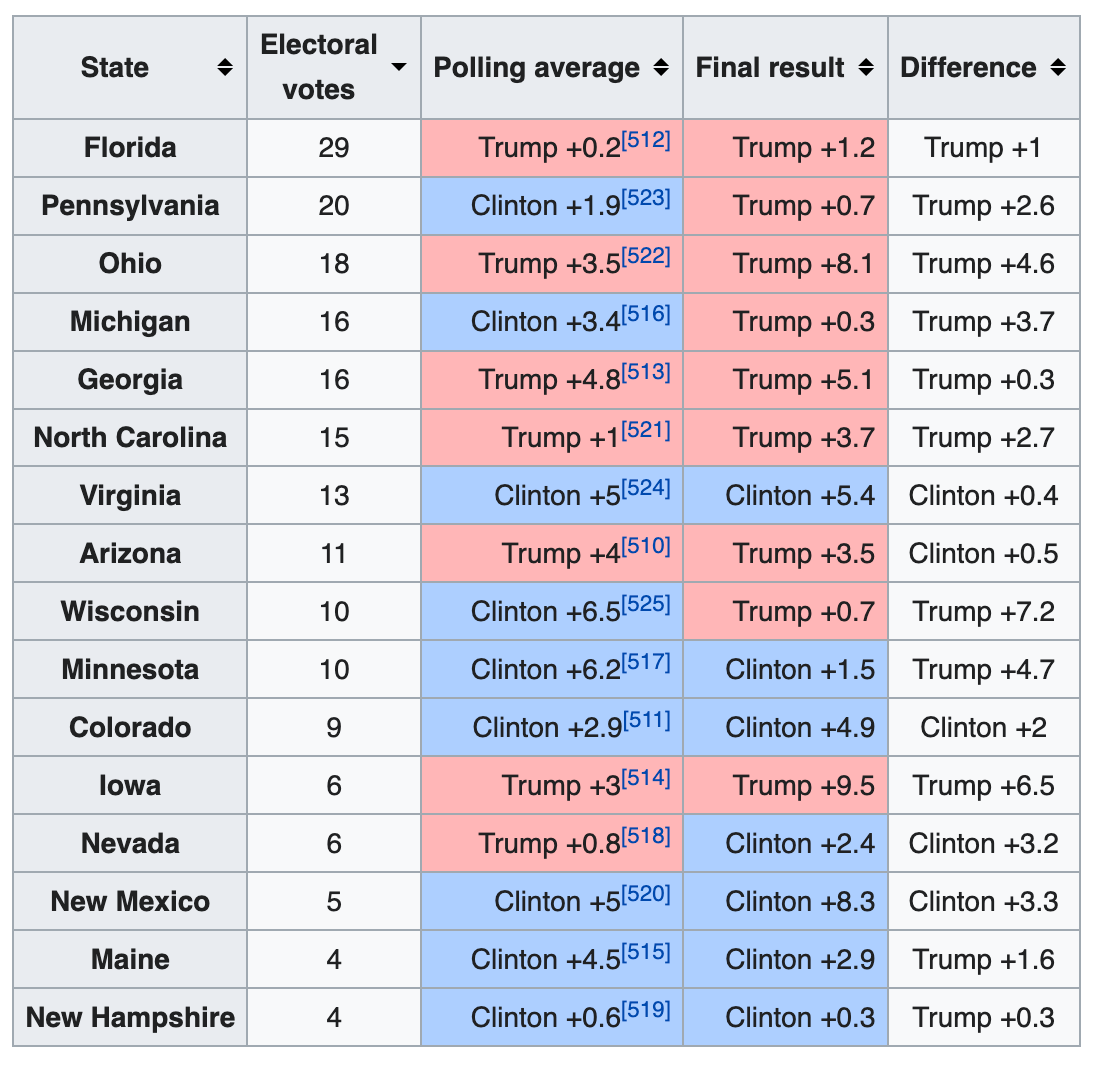
\includegraphics[scale=0.35]{polling_2016.png}
\end{center}
\end{column}
\end{columns}

\end{frame}

%@@@@@@@@@@@@@@@@@@@@@@@@@@@@@@@@@@@@@@@@@@@@@@@@@
\begin{frame}
\frametitle{Is polling good?}


\end{frame}

%@@@@@@@@@@@@@@@@@@@@@@@@@@@@@@@@@@@@@@@@@@@@@@@@@
\begin{frame}
\frametitle{Is polling good?}

\begin{itemize}
\item Polling may affect voter behavior:
\begin{itemize}
\item Bandwagoning;
\item Underdog support;
\item Turnout;
\item Strategic voting;
\end{itemize}
\bigskip
\bigskip
\bigskip

\item With plentiful (and growing) information do candidates lead or follow?

\end{itemize}

\end{frame}

%@@@@@@@@@@@@@@@@@@@@@@@@@@@@@@@@@@@@@@@@@@@@@@@@@
\begin{frame}

\begin{center}
\Huge\textbf{Why should we care?}\\
\bigskip
\bigskip
\large Polling is a core part of how modern democracy functions.\\
\end{center}

\end{frame}



\end{document}






